\hoofdstuk{Evaluation}

\begin{figure}[ht]
    \centering
    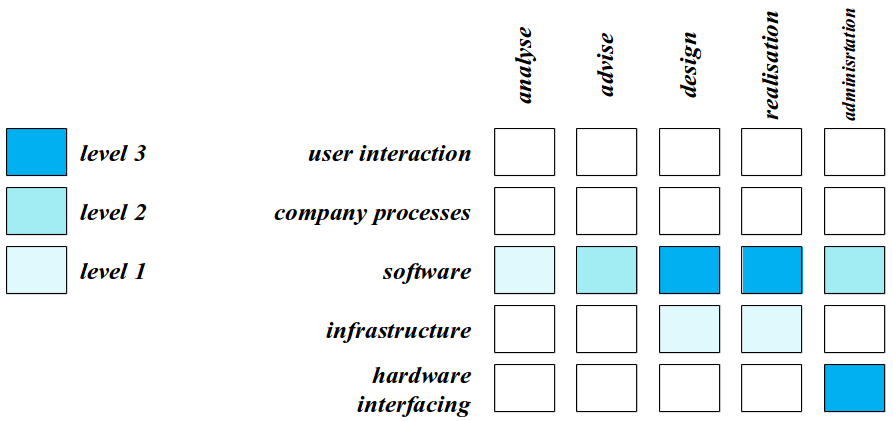
\includegraphics[width=0.8\textwidth]{plaatjes/competenties}
    \caption{Competences matrix.}
    \label{fig:top-level}
\end{figure}%

During the project which led up to this thesis, the following competences that were stated in the mandate were used. For the software category, the analyse competence was used to create the requirements necessary for the development of the application. The advice competence was used when writing the recommendations on how the application could be further improved. The design competence was necessary to design an efficient system which would fulfill the requirements. Once a design for the system has been created the application must be developed, and this is where the realisation competence comes in. Last but not least, as to prevent the loss of source code, a version control system was used. This is part of the administration competence.

Only two competences were chosen from the infrastructure category: design and realisation. To design the way the application communicated with the information website and the central application, the design competence was used. And to implement that design, the realisation competence came into play.

The last competence used was the administration competence from the hardware interfacing category. This competence was used to program the application in a way that worked within the Android platform.
